\documentclass[11pt]{article}
\usepackage{textcomp,geometry,graphicx,verbatim}
\usepackage{fancyhdr}
\usepackage{amsmath,amssymb,enumerate,cancel}
\usepackage{titling}
\setlength{\droptitle}{-10em}   % This is your set screw
\pagestyle{fancy}
\def\Name{Manohar Jois}
\def\Homework{7} % Homework number - make sure to change for every homework!
\def\Session{Spring 2015}

% Extra commands
\let\origleft\left
\let\origright\right
\renewcommand{\left}{\mathopen{}\mathclose\bgroup\origleft}
\renewcommand{\right}{\aftergroup\egroup\origright}
\newcommand{\N}{\mathbb{N}}
\newcommand{\Z}{\mathbb{Z}}
\newcommand{\R}{\mathbb{R}}
\newcommand{\Q}{\mathbb{Q}}
\newcommand{\C}{\mathbb{C}}
\newcommand{\p}[1]{\left(#1\right)}
\newcommand{\E}{\mathbb{E}}
\newcommand{\cov}{\text{Cov}}
\newcommand{\deriv}[2]{\frac{d#1}{d#2}}
\newcommand{\pderiv}[2]{\frac{\partial#1}{\partial#2}}
\newcommand{\lhood}{\mathscr{L}}
\newcommand{\sig}[1]{\text{sig}\p{#1}}
\renewcommand{\gcd}[1]{\text{gcd}\p{#1}}
\renewcommand{\deg}[1]{\text{deg}\p{#1}}
\renewcommand{\log}[1]{\text{log}\p{#1}}
\renewcommand{\ln}[1]{\text{ln}\p{#1}}
\newcommand{\logb}[2]{\text{log}_{#1}\p{#2}}
\newcommand{\BigOh}[1]{O\p{#1}}
\newcommand{\BigOmega}[1]{\Omega\p{#1}}
\newcommand{\BigTheta}[1]{\Theta\p{#1}}
\newcommand{\asdf}{\newline\newline}

\title{CS189\ \Session\  --- Homework \Homework}
\author{\Name}
\lhead{CS189\ \Session\  Homework \Homework\ Problem \theproblemnumber,\ \Name}

\begin{document}
\maketitle
\newcounter{problemnumber}
\setcounter{problemnumber}{0}

\section*{Problem 1}
\stepcounter{problemnumber}
%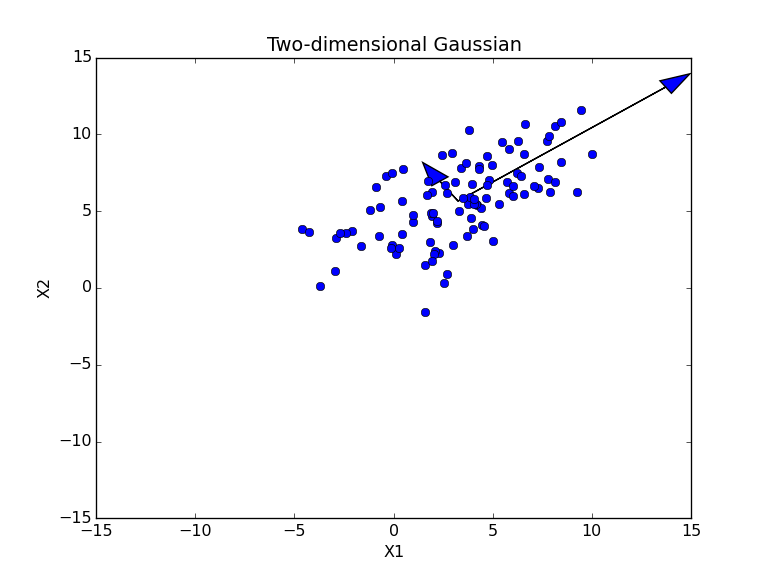
\includegraphics[scale=0.45]{images_hw3/p1d}
%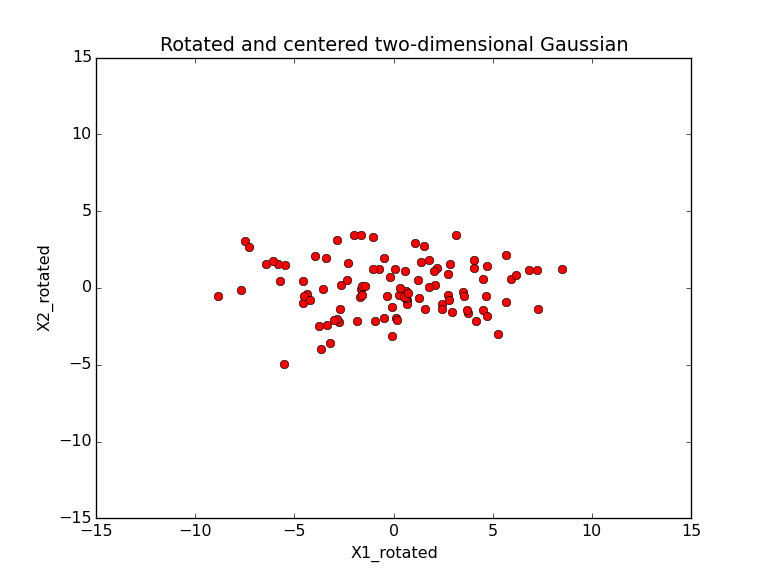
\includegraphics[scale=0.45]{images_hw3/p1e}
The cluster centers are located in the \texttt{images} directory for each run of $k$-means. Obviously the file names don't necessarily correspond to anything other than an arbitrary cluster whose formation is dependent on the random initialization. Here are the visualizations for $10$-means:\\
\begin{tabular}{cc}
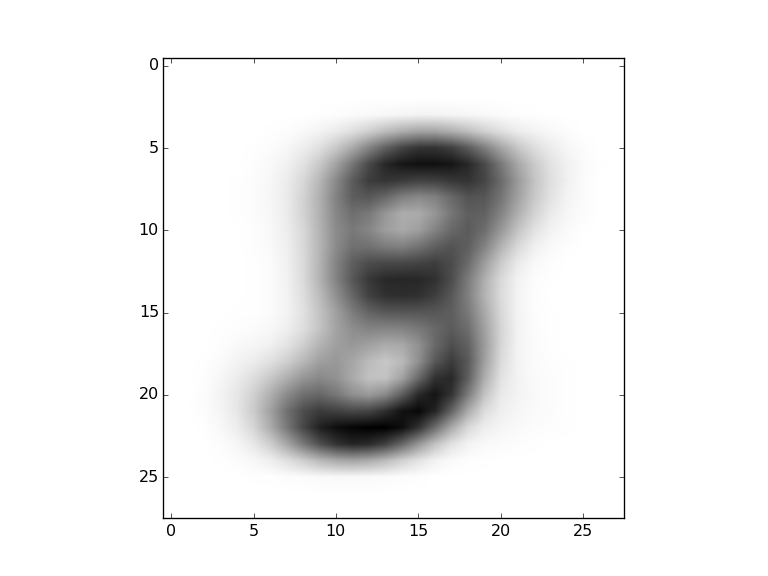
\includegraphics[scale=0.4]{images/10-images/0} & 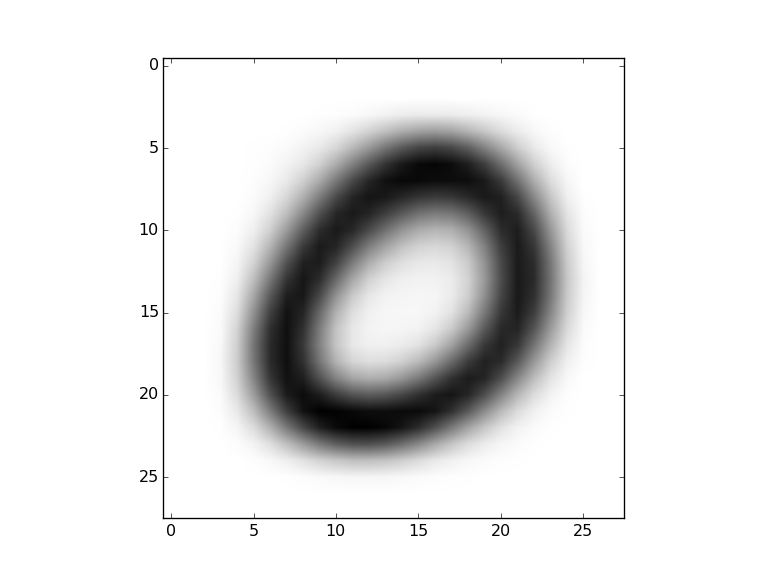
\includegraphics[scale=0.4]{images/10-images/1} \\
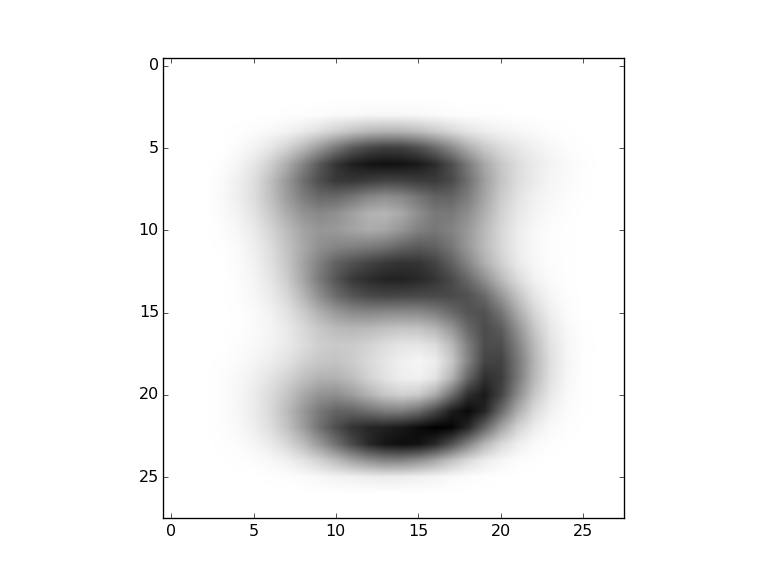
\includegraphics[scale=0.4]{images/10-images/2} & 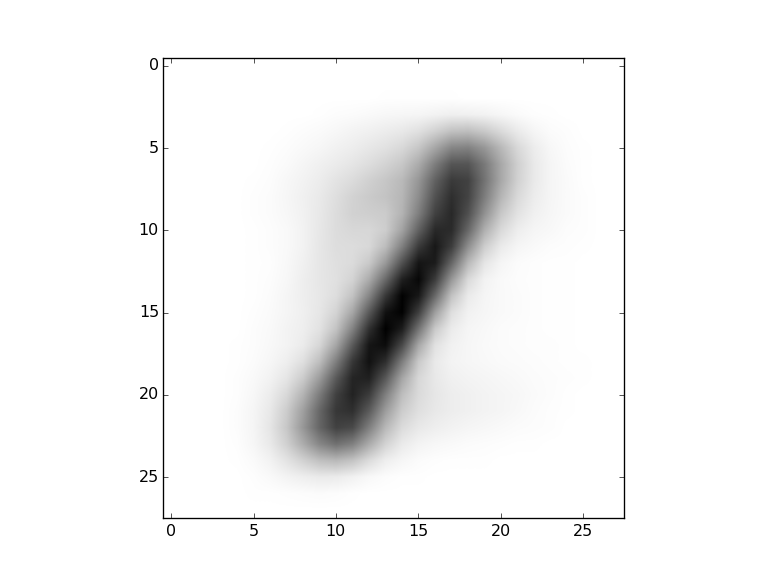
\includegraphics[scale=0.4]{images/10-images/3}
\end{tabular}
\begin{tabular}{cc}
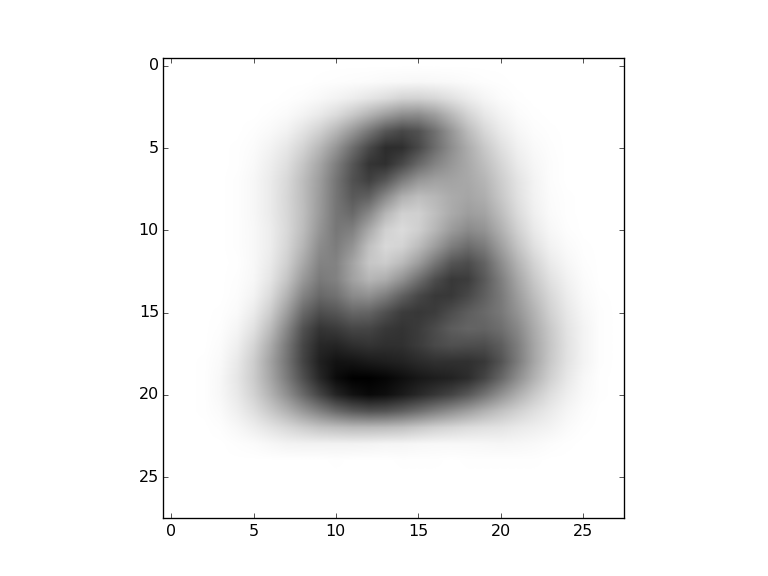
\includegraphics[scale=0.4]{images/10-images/4} & 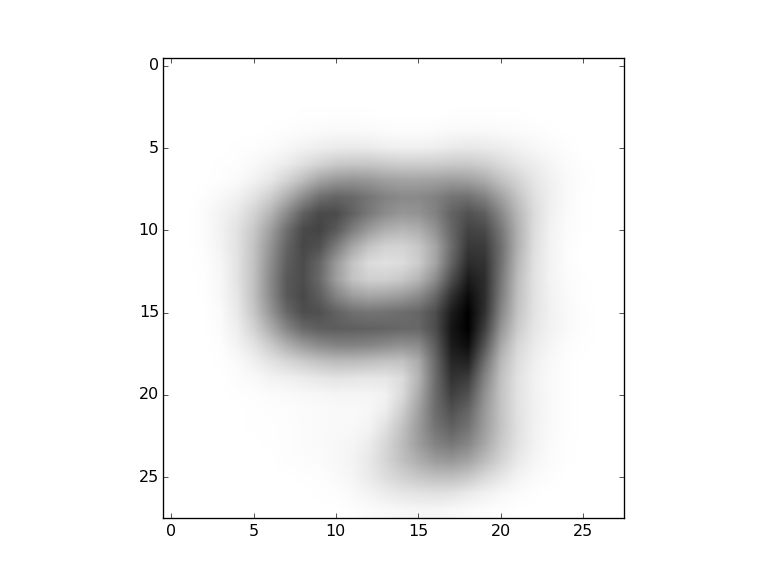
\includegraphics[scale=0.4]{images/10-images/5} \\
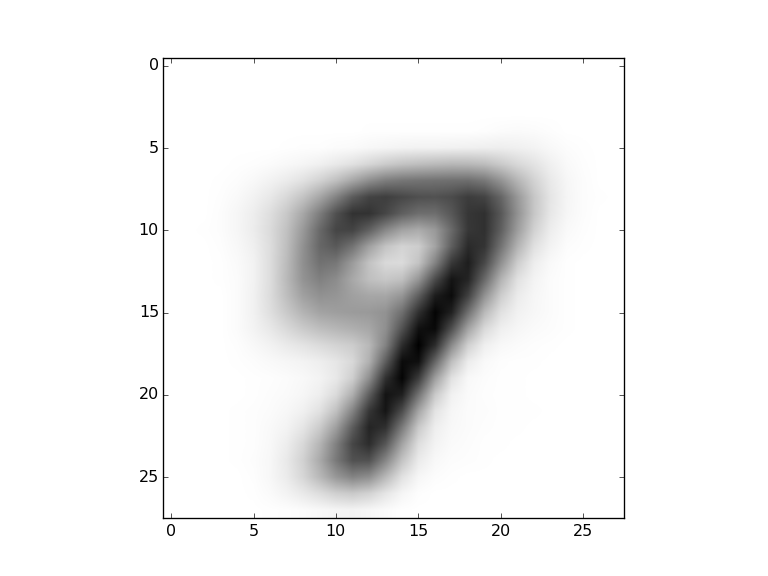
\includegraphics[scale=0.4]{images/10-images/6} & 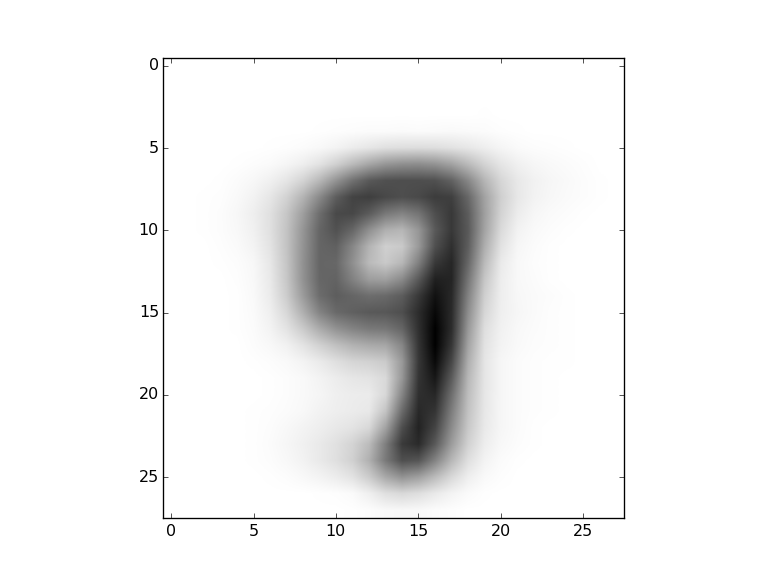
\includegraphics[scale=0.4]{images/10-images/7} \\
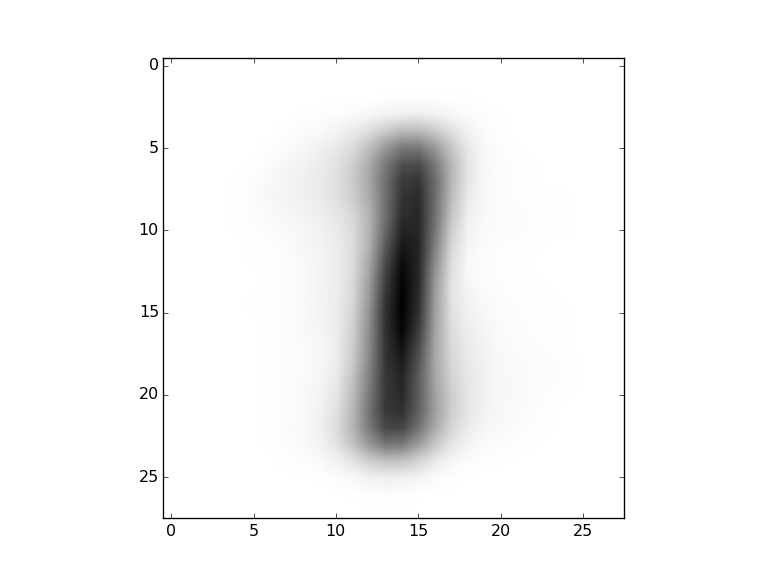
\includegraphics[scale=0.4]{images/10-images/8} & 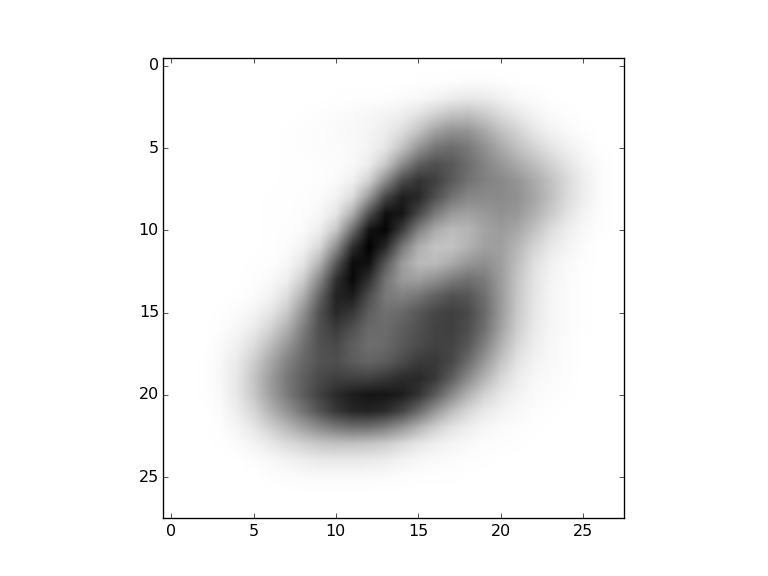
\includegraphics[scale=0.4]{images/10-images/9}
\end{tabular}\newpage
The loss can vary considerably based on the random initialization. Using $10$-means as an example, nearly all runs start with a total loss around $1.11\cdot10^8$. Some runs see this loss hover around the same value or even slightly increase, while other runs can get the loss down around $0.95\cdot10^8$.


\section*{Problem 2}
\stepcounter{problemnumber}

For the warmup, the validation accuracy for the naive rating system (average rating over all users) was about $62$ percent. For $k$-NN with $k=10,100,1000$ the validations accuracies become around $65$, $69$ and $69.5$ percent, respectively. These are certainly improvements, but they don't look to be worth the extra computational expense. Also, as we increase $k$, we essentially approach the naive rating system, and judging by these results, $k$-NN probably won't get us accuracies much higher than about $70$ percent.

\end{document}
